\subsection{RadixVM: Scalable address space operations}

The POSIX virtual memory interface is rife with commutativity, but
existing implementations scale poorly.  We model a virtual memory
system as four key logical operations: \code{mmap} adds a region of
memory to a process' virtual address space, \code{munmap} removes a
region of memory from the address space, and \code{memread} and
\code{memwrite} access virtual memory at a particular virtual address
or fail if no mapped region contains that address.  In reality, the
hardware implements \code{memread} and \code{memwrite} directly and
the VM system instead implements a \code{pagefault} operation; we
discuss this distinction below.

% Old, implementation-oriented text:
% A typical virtual memory system supports three key operations:
% \code{mmap} to add a region of memory to a process's virtual memory
% address space, \code{munmap} to remove a region of memory from the
% address space and the corresponding pages from the hardware page
% tables, and \code{pagefault}, which inserts a page into the hardware
% page tables at the faulting virtual address, allocating a new physical
% page if necessary.

% Old, more detailed memread/memwrite text:
% In reality, the hardware implements \code{memread} and \code{memwrite}
% directly using a cache of virtual-to-physical translations; when an
% operation misses in this translation cache, the hardware invokes
% \code{pagefault}, which is provided by the VM system.  This
% translation cache does not affect the interface specification or its
% commutativity; we'll discuss its effect on implementation below.

VM operations from \emph{different} processes (and hence address
spaces) trivially commute.  Most existing implementations use
per-process address space representations, so such operations are also
naturally conflict-free (and scale well).  VM operations from the same
process also often commute; in particular, operations on
\emph{non-overlapping} regions of the address space commute.
%
Many multithreaded applications exercise exactly this increasingly
important scenario: \code{mmap}, \code{munmap}, and related variants
lie at the core of high-performance memory allocators and garbage
collectors and partitioning the address space between threads is a key
design component of these
systems~\cite{ssmalloc:apsys,jemalloc,tcmalloc}.  Applications that
frequently map and unmap files also generate such workloads for the OS
kernel.

Owing to complex invariants in virtual memory systems,
widely used kernels such as Linux and FreeBSD protect each address
space with a single lock.  This induces not only conflicts but, often,
complete serialization between commutative VM operations on the same
address space, which can dramatically limit application
scalability~\cite{boyd-wickizer:scaling,clements:bonsai}.
%
As a result, applications often resort to workarounds with significant
downsides.
%
For example, a Google engineer reported to us that Google's memory
allocator is reluctant to return memory to the OS precisely because of
scaling problems with \code{munmap} and as a result applications tie
up gigabytes of memory until they exit.
%
This delays the start of other applications and can cause servers to
be used inefficiently.
%
Engineers from other companies have reported similar problems to us.

\vm is a novel virtual memory system in which commutative operations
on non-overlapping address space regions are almost always
conflict-free.  This ensures that if two threads operate on
non-overlapping
regions of virtual memory, the VM system does not limit the
application's scalability.  Furthermore, if multiple threads operate
on the same shared region, \vm constrains conflicts to the cores
executing those threads.

Achieving this within the constraints of virtual memory hardware,
without violating POSIX's strict requirements on the ordering and
global visibility of VM operations, and without unacceptable memory
overhead is challenging.  The following sections describe \vm's
approach.  \Cref{sec:radixvm:arch} describes the general architecture
of POSIX VM systems.  \Cref{sec:radixvm:tree,sec:radixvm:tlb} describe
the data structures that form the core of \vm.  Finally,
\cref{sec:radixvm:ops} describes how \vm uses these structures to
implement standard VM operations.

\subsubsection{POSIX VM architecture}
\label{sec:radixvm:arch}

\begin{figure}
  \centering
  \XXX!{Mapped regions, page tables, TLB with application on top.  See
    Bonsai Figure 1 and \vm talk.}
  \caption[Key structures in a POSIX VM system.]{Key structures in a
    POSIX VM system, showing an address space with four mapped
    regions.  Crossed-out page table entries are marked ``not
    present.''  Some pages have not been faulted yet, and thus are not
    present, despite being in a mapped region.}
  \label{fig:vm-structures}
\end{figure}

Between the POSIX VM interface on one side and the hardware virtual
memory interface on the other, \vm's general architecture necessarily
resembles typical Unix VM systems.  \Cref{fig:vm-structures} shows the
principle structures any Unix VM system must manage.  On the left is
the kernel's internal representation of the address space.  Logically,
this consists of a set of mapped regions of the virtual address space,
where each region may map either a file or ``anonymous'' heap
memory, has various access permissions, and may be either shared or
copied across \code{fork}.  \code{mmap} and \code{munmap}
manipulate this view of the address space.

Translating virtual addresses to physical addresses is
performed in hardware by the memory
management unit (MMU) and the MMU's representation of virtual memory
generally differs significantly from the kernel's internal
representation of the address space.  Most hardware architectures
specify some form of page table data structure, like the x86 page
table depicted in
\cref{fig:vm-structures}, for the kernel to inform the MMU of the
mapping from virtual addresses to physical addresses.  These
structures map addresses at a page granularity (typically 4~KB, though
most architectures also support larger pages) and represent access
permissions (which are checked by the MMU), but have little
flexibility.

While we model the VM system in terms of \code{mmap}, \code{munmap},
\code{memread}, and \code{memwrite}, only the first two are directly
implemented by the VM system.  The latter two are implemented by the
MMU using the kernel-provided page table.  However, the VM system has
a key hook into the MMU: when the virtual address of a read or a write
is marked ``not present'' in the page table or fails a permission
check, the MMU invokes the VM system's \code{pagefault} operation.
Modern Unix kernels exploit this mechanism to implement \emph{demand
  paging}, populating page table entries by allocating pages or
reading them from disk only once a page is first accessed, rather than
when it is mapped.
%
Hence, \code{mmap} and \code{munmap} simply clear the page table
entries of the region being mapped or unmapped; \code{mmap} depends on
\code{pagefault} operations to later fill these entries with mappings.
%
While demand paging significantly affects the implementation of the VM
system, it is nevertheless an implementation issue and does not affect
the commutativity of \code{memread} or \code{memwrite}.

The final key structure the VM system must manage is the hardware
translation lookaside buffer (TLB).  The TLB is a per-core associative
cache of virtual-to-physical mappings.  In architectures with a
hardware-filled TLB (x86, ARM, PowerPC, and many others), the MMU
transparently fills this cache from the page table.  Invalidating the
TLB, however, is the responsibility of the VM system.  Hence,
\code{munmap}, in addition to removing regions from the kernel's
internal address space representation and clearing entries in the page
table, must also invalidate the corresponding entries from each core's
TLB.


\subsubsection{Radix tree}
\label{sec:radixvm:tree}
\label{sec:topic:linux-coarse}

% At its core, an address space is a mapping from virtual addresses to
% physical addresses and metadata.  Hence, \vm needs a data structure
% that can track this mapping and support \code{mmap}ing and
% \code{munmap}ing ranges of virtual address space while avoiding
% conflicts between operations on non-overlapping regions.

\XXX[FK]{Maybe move parts where the radix tree violates the rule to a
  summary section (or the end of this section) that discusses how
  conflict-free \vm is?}  \XXX[AC]{Currently these things are
  discussed where they arise; if I move them to a summary I think
  people will be left wondering.}

We first tackle \vm's internal address space representation.
%
Widely-used operating system kernels represent an address space as a
balanced tree of mapped memory regions.  For example, Linux uses a
red-black tree~\cite{linux-source}, FreeBSD uses a splay
tree~\cite{freebsd-source}, and Solaris and Windows use AVL
trees~\cite{windows:wrk,windows:slides}.  This ensures $O(\log n)$ lookups
and modifications for address spaces that can easily contain thousands
of mapped regions, but these data structures are poorly suited for
concurrent access: not only do they induce cache line conflicts
between operations on non-overlapping regions, they force all of these
kernels to use coarse-grained locking.

Lock-free data structures seem like a compelling solution to this
problem.  However, while lock-free (or partially lock-free) data
structures such as the Bonsai tree used by the Bonsai
VM~\cite{clements:bonsai}, relativistic red-black
trees~\cite{howard:relrbtree}, and lock-free skip
lists~\cite{herlihy:art} eliminate the coarse-grained serialization
that plagues popular VM systems, their operations are far from
conflict-free.  For example, \code{insert} and \code{lookup}
operations for a lock-free concurrent skip list can conflict on
interior nodes in the skip list---even when the \code{lookup} and
\code{insert} involve different keys and hence commute---because
\code{insert} must modify interior nodes to maintain $O(\log n)$
lookup time.
%
The effect of these conflicts on performance can be dramatic, as shown
by the simple experiment in \cref{fig:skiplist}.
% Any balanced data structure will suffer from such problems.
Furthermore, while these data structures maintain their own integrity
under concurrent operations, a VM system must maintain higher-level
invariants across the address space representation, page tables, and
TLBs, and it is difficult to extend the precision design of a single
lock-free data structure to cover these broader invariants.

\begin{figure}
  \centering
  \input{graph/skiplist.tex}
  %
  \splitcaption{Throughput of skip list lookups with concurrent
    inserts and deletes.}{The skip list represents $\sim$1,000 virtual
    memory regions.  Lookups commute with modifications, but even a
    small number of writers significantly limits lookup scalability.}
  \label{fig:skiplist}
\end{figure}

\paragraph{Straw-man solution.}
This raises the question: what is a good conflict-free data structure
for virtual memory metadata?

A (completely impractical) way to achieve conflict-free commutative
address space
operations is to represent a process's address space as a large linear
array indexed by virtual page number that stores each virtual page's
metadata individually.
%
In this linear representation, \code{mmap}, \code{munmap},
and \code{pagefault} can lock and manipulate precisely the range of
pages being mapped, unmapped, or faulted.
%
Operations on non-overlapping regions are clearly conflict-free and
precise range locking makes maintaining invariants across structures
relatively straightforward.

\paragraph{Compressed radix trees.}
The design of \vm follows the same general
scheme as this straw-man design, but reins in its memory consumption
using a multilevel, compressed radix tree.

\begin{figure}
  \centering
  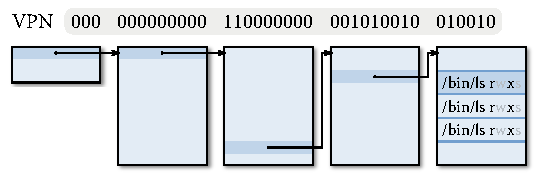
\includegraphics{figures/radix.pdf}
  %
  \splitcaption{A radix tree containing an anonymous mapping and a
    file mapping.}{Blue indicates the path for looking up the 36-bit
    virtual page number shown in bits at the top of the figure.  The
    last level of the tree contains separate mapping metadata for each
    page.  \XXX![AC]{Make this figure suck less.}}
  \label{fig:radix}
\end{figure}

\vm's internal address space representation resembles a hardware page table
structurally, storing mapping metadata in a fixed-depth radix tree,
where each level of the tree is indexed by nine or fewer bits of the
virtual page number, as shown in \cref{fig:radix}.  Like the linear array,
the radix tree supports only point queries (not range queries) and
iteration, but unlike the linear array, \vm can compress repeated
entries and lazily allocate the nodes of the radix tree.
%
The radix tree folds any node that would consist entirely of identical
values into a single value stored in the parent node.  This continues up to
the root node of the tree, allowing the radix tree to represent vast
swaths of unused virtual address space with a handful of empty slots
and to set large ranges to identical values very quickly.
%
This optimization reins in the radix tree's memory use, makes it
efficient to set large ranges to the same value quickly, and enables
fast range scans.
%
It does come at a small cost: operations that expand a subtree will
conflict with other operations in that same subtree, even if their
regions do not ultimately overlap.  However, after initial address
space construction, the radix tree is largely ``fleshed out'' and
these initialization conflicts become rare.

\paragraph{Mapping metadata.}
To record each mapping, \vm logically stores a separate instance of
the mapping metadata
in the radix tree for each page in the mapped range.  This differs
from a typical design that allocates a single metadata object
to represent the entire range of a mapping (e.g., \emph{virtual memory
areas} in Linux).
%
This is practical because \vm's mapping metadata object is small and
foldable (the mapping metadata objects of all pages in a mapped range
are initially byte-wise identical), so large mappings can be
created and stored efficiently in just a few slots in the radix tree.

Also unlike typical virtual memory system designs, \vm stores pointers
to physical memory pages in the mapping metadata for pages that have
been allocated.  This is natural to do in \vm because, modulo folding,
there is a separate mapping metadata object for each page.  It's also
important to have this canonical representation of the physical memory
backing a virtual address space because of the way \vm handles TLB
shootdown (see \cref{sec:radixvm:tlb}).  This does increase the space
required by the radix tree, but, asymptotically, it's no worse than
the hardware page tables, and it means that the hardware page tables
themselves are cacheable memory that can be discarded by the OS to
free memory.

\paragraph{Radix node garbage collection.}
To keep the memory footprint of the radix tree in check, the OS must be
able to free nodes that no longer contain any valid mapping metadata.
To accomplish this without introducing undue conflicts, we leverage
\refcache to scalably track the number of used slots in each node.
When this count drops to zero, the radix tree can remove the node from
the tree and delete it.  Since \vm may begin using a node again before
\refcache reconciles the used slot count, nodes link to their children
using weak references, which allows the radix tree to revive nodes
that go from empty to used before \refcache deletes them, and to
safely detect when an empty child node has been deleted.

Collapsing the radix tree does potentially introduce conflicts;
however, unlike with eager garbage collection schemes, rapidly
changing
mappings cannot cause the radix tree to rapidly delete and recreate
nodes.  Since a node must go unused for at least two \refcache epochs
before it is deleted, any cost of deleting or recreating it (and any
additional contention that results) is amortized.
\XXX[AC]{We don't actually implement this, but if we did, when we
analyze performance without \refcache, things would be even worse.
Might be worth mentioning.}

In contrast with more traditional balanced trees, using a radix tree
to manage address space metadata allows \vm to achieve near-perfect
conflict-freedom (and hence scalability) for metadata operations on
non-overlapping regions of an address
space.  This comes at the cost of a potentially larger memory
overhead; however, address space layouts tend to exhibit good
locality and folding efficiently compresses large ranges, making radix
trees a good fit for a VM system, as we'll confirm in
\cref{sec:eval:memory}.

\subsubsection{TLB management}
\label{sec:radixvm:tlb}

The other major impediment to scaling \code{mmap} and \code{munmap}
operations is the need to explicitly invalidate cached
virtual-to-physical mappings in per-core TLBs when a page is unmapped
(or remapped).
%
Because TLB shootdowns must be performed on every CPU that may have
cached a page mapping that's being modified, and because hardware does
not provide
information about which CPUs may have cached a particular mapping,
typical Unix VM systems conservatively broadcast TLB shootdown
interrupts to all
CPUs using the modified address space~\cite{mach:tlb}, inducing cache
line conflicts
and limiting scalability.

\vm addresses this problem by precisely tracking the set of CPUs that
have accessed each page mapping.
%
In architectures with software-filled TLBs (such as the MIPS or
UltraSPARC) this is easy, since the MMU informs the kernel of each
miss in the TLB.  The kernel can use these TLB miss faults to track
exactly which CPUs have a given mapping cached and, when a later
\code{mmap} or \code{munmap} changes this mapping, it can deliver
shootdown requests
only to cores that have accessed this mapping.  On architectures
with hardware-filled TLBs such as the x86, \vm achieves the
same effect using per-core page tables.
%
With TLB tracking, if an application thread
allocates, accesses, and frees memory on one core, with no other threads
accessing the same memory region, then \vm will perform no TLB shootdowns.

The obvious downside to this approach is the extra memory required for
per-core page tables.  We show in \cref{sec:eval:memory} that this
overhead is small in practice compared to the total memory footprint
of an application, but for applications with poor partitioning, it may
be necessary for the application to provide hints about widely shared
regions so the kernel can share page tables (similar to Corey address
ranges~\cite{boyd-wickizer:corey}) or for the kernel to detect such
regions.
%
The kernel can also reduce overhead by simply discarding page table
pages when memory is low.

\subsubsection{VM operations}
\label{sec:radixvm:ops}

With the components described above, \vm's implementation of the core
VM operations is surprisingly straightforward.
%
One of the most difficult aspects of the POSIX VM interface in a
multicore setting is its strict ordering and global visibility
requirements~\cite{clements:bonsai}.
%
For example, before \code{munmap} in one thread can return, the region
must appear unmapped to every thread on every core despite caching at
both software and hardware levels.
%
Similarly, after \code{mmap} returns, any thread on any core
must be able to access the mapped region.  Furthermore, though not
required by POSIX, it is generally assumed that these operations are
atomic.

\vm enforces these semantics by always locking, from left to right,
the bottom-most radix tree entries for the region of an operation.
%
This simple mechanism ensures that \code{mmap}, \code{munmap}, and
\code{pagefault} operations are
linearizable~\cite{herlihy:linearizability} without causing conflicts
between operations on non-overlapping regions (assuming the tree is
already expanded).

% When locking a region that has not been expanded out to leaf nodes
% yet, \vm acquires locks on the corresponding internal node slots
% instead.  When \vm expands the tree by allocating new nodes, it
% propagates the lock bit to every entry in the newly allocated node,
% and unlocks the parent interior node slot.  Releasing the lock
% clears the lock bits in the newly allocated child node.  Tree
% traversal does not require locks or indeuce conflicts because it
% increments each node's reference count through a \refcache weak
% reference.

An \code{mmap} invocation, like all \vm operations, first locks the
range being mapped.
%
If there are existing mappings within the
range, \code{mmap} unmaps them, as described later for \code{munmap}.
\code{mmap} then fills each slot in the region with the new mapping
metadata (protection
level and flags arguments to \code{mmap}, as well as what backs this virtual
memory range, such as a file or anonymous memory).
%
If parts of the mapping span entire nodes of the radix tree, \vm will
fold them into individual higher-level slots.
%
Finally, \vm unlocks the range.  Like in other VM systems,
\code{mmap}
doesn't allocate any physical pages, but leaves that to \code{pagefault},
so that pages are allocated only when they are needed.

A \code{pagefault} invocation traverses the radix tree to find the
mapping metadata for the faulting address, and acquires a lock on it.
It then allocates a physical page if one has not been allocated yet
(for anonymous memory), or fetches it from the buffer cache (for file
mappings) and
stores it in the mapping metadata.  Finally, \code{pagefault} fills in the
page table entry in the local core's page table, and adds the local core
number to the TLB shootdown list in the mapping metadata for that address.
\code{pagefault} then releases the lock and returns.

To implement \code{munmap}, \vm must clear mapping metadata from the
radix tree, clear page tables, invalidate TLBs, and free physical
pages.  \code{munmap} begins by locking the range being unmapped,
after which it can scan the region's metadata to gather references to
the physical pages backing the region, collect the set of cores that
have faulted pages in the region into their per-core page tables, and
clear each page's metadata.  It can then send inter-processor
interrupts to the set of cores it collected in the first step.  These
interrupts cause the remote cores (and the core running \code{munmap})
to clear the appropriate range in their per-core page table and
invalidate the corresponding local TLB entries.  Once all cores have
completed this shootdown process, \code{munmap} can safely release its
lock on the range and decrement the reference counts on the physical
pages that were unmapped.

% Note that an invocation of \code{pagefault} on one core may concurrently
% access a page that another core is in the process of unmapping,
% but the mapping metadata lock makes this work out correctly: either
% \code{pagefault} acquires the lock first or \code{munmap} does.  In the
% first case, the page fault succeeds, which is okay since the pages must be
% inaccessible only after \code{munmap} returns.  In the second case,
% \code{munmap} runs first and removes the mapping for the unmapped range
% before releasing the locks. Then, \code{pagefault} will see that there
% is no mapping for the faulting address and will halt the faulting thread.

\subsubsection{Discussion}

By combining \refcache for scalable reference counting, radix trees
for maintaining address space metadata, and per-core page tables for
precise TLB tracking and shootdown, \vm achieves conflict-freedom for
the vast majority of commutative VM operations.  The clear
commutativity properties of the POSIX VM interface, combined with the
right data structures makes this possible with a straightforward
concurrency plan based on precise range locking.

\vm balances practical memory consumption with strict adherence to
scalable commutativity rule, allowing conflicts between some
commutative operations where doing so enables far more efficient
memory use.  However, such conflicts are rare: operations that
allocate a radix node will conflict with later operations on that
node's range of the key space, but typical address space usage
involves few node-allocating operations.

As shown in \cref{fig:testcase-breakdown-sv6}, \tool confirmed that
most commutative operations in \vm are conflict-free.  In
\cref{sec:eval}, we further confirm that \vm's design translates into
scalable performance for application workloads.
